\documentclass[letter,11pt,oneside]{article}
%%% HEREHEREHERE
%%% APPENDIX
%%% (insert (format "\n%% %s\n" (buffer-file-name)))
% /home/git/external/FlexBerry/documentation/tex/PuttyXMingDoc/PuTTYXmingPDF.tex


%%% (occur "\\(\\\\[a-z]*section\\|appendix\\|input\\|\\<include\\>\\)")

%%\documentclass[11pt,twocolumn]{article}
%%\usepackage[inline]{asymptote}       %% Inline asymptote diagrams
%%\usepackage{wglatex}                 %% Use this one and kill others.
\usepackage{xcolor}                     %% colored letters {\color{red}{{text}}
\usepackage{fancybox}              %% headers/footers
\usepackage{fancyhdr}                  %% headers/footers
\usepackage{datetime}                  %% pick up tex date time 
\usepackage{lastpage}                  %% support page of ...lastpage
\usepackage{times}                     %% native times roman fonts
\usepackage{textcomp}                  %% trademark
\usepackage{amssymb,amsmath}           %% greek alphabet
\usepackage{parskip}                   %% blank lines between paragraphs, no indent
\usepackage{shortvrb}                  %% short verb use for tables
\usepackage{lscape}                    %% landscape for tables.
\usepackage{longtable}                 %% permit tables to span pages wg-longtable
\usepackage{multicol}                  %% Enhance footnotes/endnotes
\usepackage{url}                       %% Make URLs uniform and links in PDFs
\usepackage{enumerate}                 %% Allow letters/decorations for enumerations
\usepackage{endnotes}                  %% Enhance footnotes/endnotes
\usepackage{listings}                  %% Make URLs uniform and links in PDFs
\pdfadjustspacing=1                    %% force LaTeX-like character spacing
\usepackage{geometry}                  %% allow margins to be relaxed
%%\usepackage{wrapfig}                 %% permit wrapping figures.
%%\usepackage{subfigure}               %% images side by side.
\geometry{margin=1in}                  %% Allow narrower margins etc.
\usepackage[T1]{fontenc}               %% Better Verbatim Font.
\renewcommand*\ttdefault{txtt}        %% 
\usepackage[colorlinks=true]{hyperref} %% Make huperlinks within a PDF
\renewcommand*\ttdefault{txtt}     %%
\usepackage{natbib}                    %% bibitems
\usepackage{upquote}                   %% make programmer's quoetes in verbatim sections.

%% include background image (wg-document-page-background) 

\usepackage{graphicx}            %% Include pictures into a document
%% (wg-texdoc-inserttikz)


\def\documentisdraft{DRAFT}

%% (wg-texdoc-isdraft)


\def\drafttest{DRAFT}
\def\wgdocdate{25 Aug, 2023}
\def\wgdocdatetime{\wgdocdate at \currenttime}
\ifx\documentisdraft\drafttest
\usepackage[left]{lineno}   %%%%%%%%%%%%% DRAFT
\usepackage{draftwatermark}
%%\SetWatermarkScale{5.0}
%%\SetWatermarkColor[gray]{0.3}
\fi

%% (wg-texdoc-insert-fancy-headers)

%%\usepackage[bookmarks]{hyperref} %% Make huperlinks within a PDF
%%\usepackage{makeidx}             %% Make an index uncomment following line
%%\makeindex                       %%.. yeah this one, too. index{key} in text
%%

\makeatletter
\newcommand\llbox[1]{%
  \@tfor\@ii:=#1\do{%
    {\color{verbcolor}\Ovalbox{\strut\@ii}}%
  }%
}
\makeatother


\definecolor{verbcolor}{rgb}{0.6,0,0}
\definecolor{darkgreen}{rgb}{0,0.4,0}
\newcommand\debate[1]{\textcolor{darkgreen}{DEBATE: #1} \marginpar{\textcolor{red}{DEBATE} }}
\newcommand{\ltodo}[2]{\marginpar{\textcolor{red}{ACTION: #1}\endnote{#2}}}
\renewcommand{\thefigure}{\thesection-\arabic{figure}}
\newcommand{\menu}{\ensuremath{\;\rightarrow\;}}
\newcommand{\dhl}[1]{{\color{verbcolor}{\texttt#1}}}
\definecolor{wglightgreen}{rgb}{0.88, 0.58, 0.88}
\newcommand{\wgtextbox}[1]{\noindent\fcolorbox{darkgreen}{wglightgreen}{%
    \minipage[t]{\dimexpr0.80\linewidth-2\fboxsep-2\fboxrule\relax}
        {#1}
    \endminipage}}

%%(wg-latex-snippet)

%%(wg-add-inline-images)  %% add inline images to the mix




%%Begin User Definitions: Hint: ~/.latex.defs and  latex.defs  
%%End User Definitions:

%% (wg-texdoc-adjust-paper-width)
%% (wg-texdoc-insert-hypersetup)

%%% PDF Fields uncomment \usepackage[bookmarks]{hyperref} above.
\hypersetup{
colorlinks=true,
linkcolor=blue,
citecolor=red,
urlcolor=blue,
pdfauthor = {Copyright(c) 2020. All rights reserved. Wayne Green},
pdftitle = {A TeX Document},
pdfsubject = {My Subject Stuff here},
pdfkeywords = {Keyword1, Keyword2, ...},
pdfcreator = {LaTeX with hyperref package},
pdfproducer = {dvips + ps2pdf}}

%% (wg-latex-tablet-page)


%%%%%%%%%%%%%%%%%%%%%%%%%%%%%%%%%%%%%%%%%%%%%%%%%%%%%%%%%%%%%%%%%%%%%%%%%%%%%


\begin{document}


%% (wg-latex-pretty-title-page)
%% (wg-texdoc-titleblock)


\title{FlexSpec1 Manual Arduino Control with PuTTY and Xming on Windows}
\author{Wayne Green}
\settimeformat{hhmmsstime}
\date{\today ~ ~ \currenttime~ MT}
\maketitle

%%\begin{abstract}
This document covers using a Win1X machine to control a Raspberry Pi
over the Internet.

As of October 2023 we are leaning to using the
StellarMate\footnote{\url{https://stellarmate.com/}} product together
with PuTTY\footnote{\url{https://www.putty.org/}}\footnote{\dhl{sudo
    apt install putty -y}}. These notes were developed for for our
roll-your-own interface.

Stellarmate package has many support features already installed. Jasem
Mutlaq, the author, is heavily involved with Kstars, libindi and Ekos
-- so the integration is very strong. We have successfully used the
package in both stand-alone mode on the Raspberry Pi (RPi), with
X-Windows
XMing\footnote{\url{https://sourceforge.net/projects/xming/}} support,
in its 'split' mode -- where a basic interface is provided between a
Win1X system and a remote libinbdi-server running on the RPi. As of
October 2023 we tested between Boulder CO, Phoenix AZ, Portland OR and
Newcastle upon Tyne, UK.


%%\end{abstract}
\begin{table}[h!]
\centering
\begin{tabular}{| l | l | l |}
\hline
Service           & Port            &  WAN/Internet Control        \\ 
\hline
SSH               & 5624            & Required for Flexspec        \\ 
INDI Web Manager  & 8624            & Not required                 \\ 
INDI Server       & 7624            & Not required                 \\ 
EkosLive Server   & 3000            & Not required                 \\ 
Web VNC           & 6080            & Not required                 \\ 
VNC               & 5900            & Not required                 \\ 
Serial            & /dev/ttyS<n>    & Arduino Serial1 pins on RPi  \\ 
Serial            & /dev/ttyACM0    & Arduino Serial USB           \\ 
\hline
\end{tabular}
\caption[Stellarmate Wan Ports]{Stellarmate Wan Firewall Requirements}
\end{table}


%%%%%%%%%%%%%%%%%%%%%%%%%%%%%%%%%%%%%%%%%%%%%%%%%%%%%%%%%%%%%%%%%%%%%%%%%%%%%
%% table of contents
%%%%%%%%%%%%%%%%%%%%%%%%%%%%%%%%%%%%%%%%%%%%%%%%%%%%%%%%%%%%%%%%%%%%%%%%%%%%%
 
\pagenumbering{roman}   % i,ii,etc
%%\pagenumbering{gobble}   %ignore page numbers for a while
\pdfbookmark[0]{Table of Contents}{MyTOC} % if usepackage{hyperref} in use.
\tableofcontents
\listoffigures
%\listoftables
\newpage


\setcounter{section}{0}
\pagenumbering{arabic}


\ifx\documentisdraft\drafttest
\linenumbers    %%%%%%%%%%%%% DRAFT
\fi

% PuTTYXming.tex

\section*{PuTTY and Xming on Windows} \label{sec:puttyxming}
\setcounter{section}{1}

PuTTY running remotely on a Raspberry Pi uses X11 to share its
interface with the remote user. This may require XMing for Win11, and
XQuartz for Apple machines. It may require including a X11 desktop (in
lieu of Wayland) on the remote Linux machines.

This article addresses executing PuTTY on a Raspberry Pi from a Win1X
machine located elsewhere on the Internet. It addresses basic tactical
aspects of network configuration. Direct X11 and port-to-port TCP
methods sidestep the bandwidth overhead of VNC like environments.  The
office desktop is presumed to be a Win1X office desktop, but may be a
Linux desktop with built-in native X11 protocols\footnote{In X11, the
  XClient is the program with all the builtin domain/control logic --
  like a spreadsheet, that offers up a GUI connection. An XServer,
  with all the logic for window creation, managing user interaction
  and 'serving' back graphics etc ties the user to the XClient's
  logic. The XServer may be elsewhere on the network from the running
  program. The protocol is very light-weight compared to
  remote-desktop (VNC) methods.}\footnote{Note: The Wayland
  X11-Replacement may introduce X11 issues.}, or an Apple machine with
a proper X11 Server support package like XQuartz.  Linux is addressed
in section \ref{sec:PuttyLinuxDesktop}.

Win1X requires an X11 Server support program. Here the
Xming\footnote{Get Xming: https://sourceforge.net/projects/xming/} package is the
only one discussed.

The typographic conventions used in these notes.

Here \llbox{k} means hit the ``k'' on the keyboard. 

For the Win1X office desktop, it is important that you acquire and install:
\vspace{-.15cm}
\begin{enumerate}\addtolength{\itemsep}{-0.5\baselineskip}
%\setcounter{enumi}{N}
   \item   Win1X office desktop
\vspace{-.15cm}
\begin{enumerate}\addtolength{\itemsep}{-0.5\baselineskip}
%\setcounter{enumi}{N}
   \item   XMing
   \item   PuTTY
\end{enumerate}
   \item   Raspberry Pi
\vspace{-.15cm}
\begin{enumerate}\addtolength{\itemsep}{-0.5\baselineskip}
%\setcounter{enumi}{N}
   \item   PuTTY
\end{enumerate}
   \item   Optional Linux office desktop
\vspace{-.15cm}
\begin{enumerate}\addtolength{\itemsep}{-0.5\baselineskip}
%\setcounter{enumi}{N}
   \item   PuTTY
\end{enumerate}
\end{enumerate}

You need to configure XMing's XLaunch program. You need to configure the
Raspberry Pi's configuration.


The PuTTY program provides a X11/ssh connection to remote machines. Here
the machine's hostname is \dhl{stellarmate.local}, the port is 22.

Xming is a X11 ``server'' (meaning is backwards from a data center's
client/server sense). X11 ``serves'' the graphics from a remote machine
doing all the heavy computing on a light-weight machine that knows nothing
about the remote application.

Grab Xming and install on a Win machine.

First some X11 magic:

You will open a \dhl{ssh -X} connection to the Raspberry Pi. This
allows linux to display a console window on the Win1X office desktop
monitor. In that window (remember will start programs on the Raspberry
Pi) you will start a PuTTY program running on the Raspberry Pi that
causes its window to appear on the Win1X office desktop.

\begin{figure}[h!]
\centering
\includegraphics[width=.5\textwidth]{images/PuTTYDiagram1.png}
\caption[Win1X use.]{Win1X office desktop monitor uses TCP/IP and SSH
  with the -X switch to open a connection to Raspberry Pi. A PuTTY
  instance is started on the Raspberry Pi, configured for the USB port
  for the Arduino displays the PuTTY window on the remote desktop vi
  SSH -X working with Xming} %% \caption{{\tiny{citation}}}
\label{figure:Diagram1}
\end{figure}

\begingroup \fontsize{10pt}{10pt}
\selectfont
%%\begin{Verbatim} [commandchars=\\\{\}]
\begin{verbatim} 

Check the files in the /etc/X11 directory:
   /etc/X11/xinit/xserverrc
   ~/.xinitrc
   ~/.xsession  -- start programs when the login is complete
   ~/.profile

ssh-keygen -t ed25519 -C "your_email@example.com"

\end{verbatim}
\endgroup
%% \end{Verbatim}

If there is no /etc/X11


\verb=xmodmap -pke > ~/.Xmodmap # make a .Xmodmap upon which to hack=

This varies with new modern keyboards, there is massive
confusion over what a key is called and what code corresponds to
the key among keyboard vendors. 

To use the \dhl{caps lock} key as a spare \dhl{control} key find the
code for the caps lock key using the \dhl{xev} program. Xev will show
keycodes when a key changes state, like shift down, then shift up
etc...  

Hit the the ``caps'' key and note its code. Then edit the \dhl{~/.Xmodmap}
file and change:

\verb/keycode  37 = Control_L NoSymbol Control_L/



\newpage
\subsection{Remote Desktop PuTTY}

On the remote desktop, configure the remote PuTTY:

\vspace{-.15cm}
\begin{enumerate}\addtolength{\itemsep}{-0.5\baselineskip}
%\setcounter{enumi}{N}
   \item   Session:
\vspace{-.15cm}
\begin{enumerate}\addtolength{\itemsep}{-0.5\baselineskip}
%\setcounter{enumi}{N}
   \item   Select the \dhl{Serial} radio button
   \item   Serial Line to \dhl{/dev/ttyACM0}
   \item   Speed \dhl{9600}
   %\item   CTM\_X
   \item   Close window on exit $\rightarrow$ \dhl{Only on clean exit}
\end{enumerate}
   \item   Terminal
\vspace{-.15cm}
\begin{enumerate}\addtolength{\itemsep}{-0.5\baselineskip}
%\setcounter{enumi}{N}
   \item   In the \dhl{Line disipline options}:
\vspace{-.15cm}
\begin{enumerate}\addtolength{\itemsep}{-0.5\baselineskip}
%\setcounter{enumi}{N}
   \item  Local echo to \dhl{Force on}
   \item  Local line editing to \dhl{Force on}
\end{enumerate}
\end{enumerate}
   \item   Window
\vspace{-.15cm}
\begin{enumerate}\addtolength{\itemsep}{-0.5\baselineskip}
%\setcounter{enumi}{N}
   \item   Columns: \dhl{120} Rows: \dhl{50}
   \item   scrollback 200
   \item   display scrollbar
   %\item   Reset scrollback on display activity
   %\item   push erased text into scrollback
\end{enumerate}
   \item   Connection $\rightarrow$ Data
\vspace{-.15cm}
\begin{enumerate}\addtolength{\itemsep}{-0.5\baselineskip}
%\setcounter{enumi}{N}
   \item   login name can be set to \dhl{stellarmate} for stellarmate, or
     the remote user's name.
   \item   Terminal-type string xterm
   \item   Terminal Speed 38400, 38400
\end{enumerate}
\item SSH
\vspace{-.15cm}
\begin{enumerate}\addtolength{\itemsep}{-0.5\baselineskip}
%\setcounter{enumi}{N}
   \item   Remote Command to \dhl{/home/stellarmate/bin/flex.py}
\end{enumerate}

   \item   SSH$\rightarrow$X11

\vspace{-.15cm}
\begin{enumerate}\addtolength{\itemsep}{-0.5\baselineskip}
%\setcounter{enumi}{N}
   \item   Enable X11 forwarding
   \item   localhost:0.0
   \item   MIT-Magic-Cookie-1
\end{enumerate}
\vspace{-.15cm}
\begin{enumerate}\addtolength{\itemsep}{-0.5\baselineskip}
%\setcounter{enumi}{N}
   \item   Serial
\vspace{-.15cm}
\begin{enumerate}\addtolength{\itemsep}{-0.5\baselineskip}
%\setcounter{enumi}{N}
   \item   Baud to 9600
   \item   Data bits 8
   \item   Stop bits 1
   \item   Parity None
   \item   Flow Control None.
\end{enumerate}
\end{enumerate}

\end{enumerate}

\begin{figure}[h!]
\centering
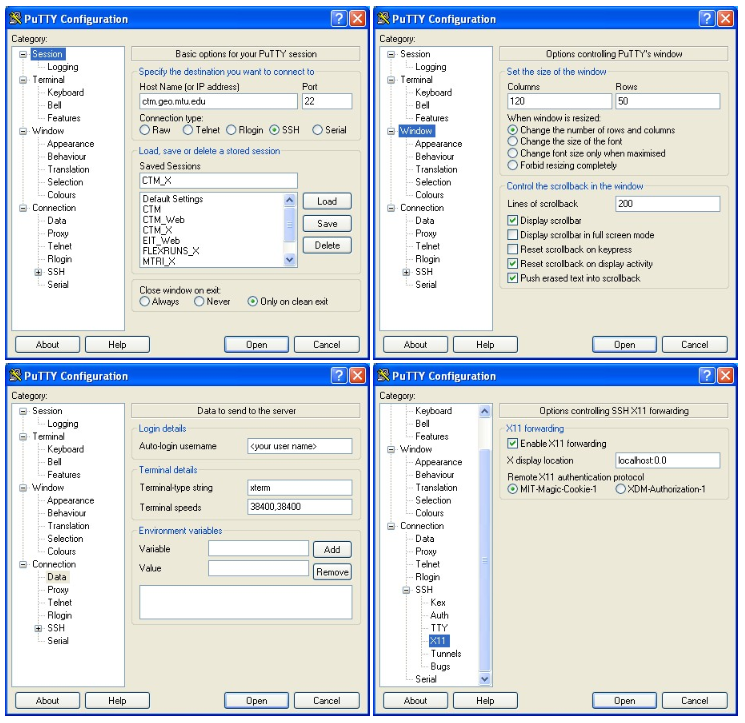
\includegraphics[width=.7\textwidth]{images/PuYYTXming.png}
\caption{PuTTY screen snaps of the 4 configuration menu panels.} %% \caption{{\tiny{citation}}} 
\label{figure:PuYYTXming}
\end{figure}



\newpage
\subsection{Remote Desktop Xming}


On the Windows pane, enter a new configuration for this machine.

\vspace{-.15cm}
\begin{enumerate}\addtolength{\itemsep}{-0.5\baselineskip}
%\setcounter{enumi}{N}
   \item Page 1 - Set Multiple windows (Each remote application gets
     its own Win1X office desktop window).
   \item Page 2 - Start no client. The clients are started with the
     Win1X PuTTY's SSH -X session.
   \item  Page 3 - Clipboard (handy)
   \item Page 4 - Save the configuration. This sets the policy for all
     machines, Xming does not care about the remote machines business
     -- any remote may connect if firewall permissions are set.
\end{enumerate}


\begin{figure}[h!]
\centering
\includegraphics[width=.75\textwidth]{images/XmingConfig.png}
\caption{Xming screen snaps of the 4 configuration menu panels.} %% \caption{{\tiny{citation}}} 
\label{figure:XmingConfig}
\end{figure}


Details for the Raspberry Pi.

\newpage
\section{Raspberry Pi}

Details related to the Raspberry Pi.


\subsection{SSH on Raspberry Pi}

The StellarMate image has all necessary ports open and ready for use.
The firewall has been set to pass all relevant ports.

See subsection \ref{sec:StellarMate} below.

\subsection{Non-StellarMate Raspberry Pi's}

Note: this section is complicated by the details needed to open
home firewalls to the internet using the local Telco's interface
routers. Each router is different, and the Telco changes its mind
frequently.

This command will list the full name for hosts that are on the network.
Here we're looking for our machine \dhl{pier15} that will appear
as \dhl{pier15.hsd1.co.comcast.net}:

{\color{verbcolor}{\verb={sudo nmap -sP 10.1.10.0/24 | awk -e '/^Nmap/ {print $5;}'}=}}

If ssh issues a:

\dhl{ssh: connect to host <machine>.local port 22: Connection refused}

use the keyboard/mouse for the raspbian machine and run the command
\dhl{sudo raspi-config}, then under Interface options, \dhl{I2 SSH} \llbox{{TAB}}, enable.


SSH (Secure SHell), originates on port 22. The port needs to be allowed
through the Raspbian's ``uncomplicated firewall'' \dhl{ufw} task. Root
permissions are required.

\begingroup \fontsize{10pt}{10pt}
\selectfont
%%\begin{Verbatim} [commandchars=\\\{\}]
\begin{verbatim} 
sudo ufw list       # see all the current ports
sudo ufw allow ssh  # allow the port to work.
\end{verbatim}
\endgroup
%% \end{Verbatim}

\subsection{Raspberry Pi -- Raspbian SSH}

Enable SSH through the Raspberry Pi Configuration menu:
\dhl{Preferences $\rightarrow$ Raspberry Pi Configuration} Click on ``Interfaces'':
and select \dhl{Enabled} next to SSH.

Use the command \dhl{sudo nano /etc/ssh/sshd\_config} find
and X11Forwarding set the value to yes 

\dhl{ X11Forwarding yes}.

Save.

\dhl{sudo systemctl restart ssh}

% https://techsphinx.com/raspberry-Pi/enable-x11-forwarding-on-raspberry-Pi/

\subsection{Serial Ports}

At end of file:

\begingroup \fontsize{10pt}{10pt}
\selectfont
%%\begin{Verbatim} [commandchars=\\\{\}]
\begin{verbatim} 
dtoverlay=disable-bt
dtoverlay=uart1
dtoverlay=uart2
droverlay=uart3
dtoverlay=uart4
dtoverlay=uart5
\end{verbatim}
\endgroup
%% \end{Verbatim}

Pinouts:

\begingroup \fontsize{10pt}{10pt}
\selectfont
%%\begin{Verbatim} [commandchars=\\\{\}]
\begin{verbatim} 
0/1    14/15   Same Uart
2       0/1
3       4/5
4       8/9
5      12/13
\end{verbatim}
\endgroup
%% \end{Verbatim}


To disable the Bluetooth 

\dhl{sudo systemctl disable hciuart}

\dhl{/boot/cmdline.txt:}

add \dhl{console=ttyS0,115200} to the main line.

\newpage
\subsection{Raspberry External Pin Functions}

\begingroup \fontsize{10pt}{10pt}
\selectfont
%%\begin{Verbatim} [commandchars=\\\{\}]
\begin{verbatim} 
  ALT0       ALT1       ALT2       ALT3       ALT4       ALT5      
 0 SDA0       SA5        PCLK       SPI3_CE0_N TXD2       SDA6      
 1 SCL0       SA4        DE         SPI3_MISO  RXD2       SCL6      
 2 SDA1       SA3        LCD_VSYNC  SPI3_MOSI  CTS2       SDA3      
 3 SCL1       SA2        LCD_HSYNC  SPI3_SCLK  RTS2       SCL3      
 4 GPCLK0     SA1        DPI_D0     SPI4_CE0_N TXD3       SDA3      
 5 GPCLK1     SAO        DPI_D1     SPI4_MISO  RXD3       SCL3      
 6 GPCLK2     SOE_N      DPI_D2     SPI4_MOSI  CTS3       SDA4      
 7 SPI0_CE1_N SWE_N      DPI_D3     SPI4_SCLK  RTS3       SCL4      
 8 SPI0_CE0_N SDO        DPI_D4     _          TXD4       SDA4      
 9 SPI0_MISO  SD1        DPI_D5     _          RXD4       SCL4      
10 SPI0_MOSI  SD2        DPI_D6     _          CTS4       SDA5      
11 SPI0_SCLK  SD3        DPI_D7     _          RTS4       SCL5      
12 PWM0       SD4        DPI_D8     SPI5_CE0_N TXD5       SDA5      
13 PWM1       SD5        DPI_D9     SPI5_MISO  RXD5       SCL5      
14 TXD0       SD6        DPI_D10    SPI5_MOSI  CTS5       TXD1      
15 RXD0       SD7        DPI_D11    SPI5_SCLK  RTS5       RXD1      
16 FL0        SD8        DPI_D12    CTS0       SPI1_CE2_N CTS1      
17 FL1        SD9        DPI_D13    RTS0       SPI1_CE1_N RTS1      
18 PCM_CLK    SD10       DPI_D14    SPI6_CE0_N SPI1_CE0_N PWM0      
19 PCM_FS     SD11       DPI_D15    SPI6_MISO  SPI1_MISO  PWM1      
20 PCM_DIN    SD12       DPI_D16    SPI6_MOSI  SPIl_MOSI  GPCLK0    
21 PCM_DOUT   SD13       DPI_D17    SPI6_SCLK  SPI1_SCLK  GPCLK1    
22 SD0_CLK    SD14       DPI_D18    SD1_CLK    ARM_TRST   SDA6      
23 SD0_XMD    SD15       DPI_D19    SD1_CMD    ARM_RTCK   SCL6      
24 SD0_DATO   SD16       DPI_D20    SD1_DAT0   ARM_TDO    SPI3_CE1_N
25 SD0_DAT1   SD17       DPI_D21    SD1_DAT1   ARM_TCK    SPI4_CE1_N
26 SD0_DAT2   TE0        DPI_D22    SD1_DAT2   ARM_TDI    SPI5_CE1_N
27 SD0_DAT3   TE1        DPI_D23    SD1_DAT3   ARM_TMS    SPI6_CE1_N
\end{verbatim}
\endgroup
%% \end{Verbatim}




\subsection{StellarMate} \label{sec:StellarMate}

You need to \dhl{sudo apt update}, then \dhl{sudo apt install putty -y}
to install PuTTY.

Add the \dhl{x11-utils} package to pick up the rather silly command
xeys. This displays two white eyeballs and the pupils track the mouse
movement. While small and cute, it does a rather deep test of the X11
capability including managing the event manager. This is helpful
to debug X11 connnections.

\begin{quote}
\dhl{sudo apt install -y x11-utils}
\end{quote}

Other programs:
\begin{quote}
\dhl{sudo apt install -y saoimage-ds9}  \\
\dhl{sudo apt install -y iraf}          \\ 
\dhl{sudo apt install -y python3-pyraf}
\end{quote}


The ssh connect to StellarMate is made to an alternate port:

\dhl{ssh -X -p 5624 stellarmate@stellarmate.local}

The username is \dhl{stellarmate} and the password is the usual
StellarMate password.

\section{Using Putty from Linux Desktop} \label{sec:PuttyLinuxDesktop}

PuTTY on a linux desktop machine in the office has all the Xming features
built-in and does not require additional X-windows code.

\section{Linux Ports}

devices such as serial ports, USB ports etc appear simply as
filenames.  For example the Arduino often identifies as
\dhl{/dev/ttyACM0}. By making no distinction using devices becomes
very easy but drives Win1X people nuts.

See section \ref{sec:RPiSerialPorts} for details about the Raspberry Pi.

The ports you are interested in:

\vspace{-.15cm}
\begin{enumerate}\addtolength{\itemsep}{-0.5\baselineskip}
%\setcounter{enumi}{N}
   \item   /dev/serial0 - the serial port pins on the Raspberry Pi. This requires 
special action to enable the GPIO pins. This is recognized by the Arduino on its Serial1
 device.
   \item   /dev/ttyAMC0 - the USB port recognized by the Arduino on its Serial
 device.
\end{enumerate}

\section{Running the Arduino CLI on the Raspberry Pi}

The Raspberry Pi will run the Arduino CLI, which in turn may run a
serial port connection. Using the magic of X11, discussed above, the
Arduino CLI windows will appear on the Win1X office desktop monitor or
Linux office desktop monitor.

From the Win1X machine:

\vspace{-.15cm}
\begin{enumerate}\addtolength{\itemsep}{-0.5\baselineskip}
%\setcounter{enumi}{N}
   \item   Use Xlaunch with multiple windows.
   \item   Then make a PuTTY connection to the RPi. (Call this Win1X/Rpi)
\vspace{-.15cm}
\begin{enumerate}\addtolength{\itemsep}{-0.5\baselineskip}
%\setcounter{enumi}{N}
   \item   this opens a Win1X cmd window, and prompts for the password into
 the RPi machine.
   \item   A Rpi prompt will appear.
\end{enumerate}

   \item   In the Win1X/Rpi window (now a shell on the RPi)
\vspace{-.15cm}
\begin{enumerate}\addtolength{\itemsep}{-0.5\baselineskip}
%\setcounter{enumi}{N}
   \item   enter the command \dhl{putty {-}{-}display=\$DISPLAY} (two dashes)
   \item   This causes a PuTTY configuration window from the RPi to appear on the 
           Win1X desktop.
   \item   Configure for the serial connection desired \dhl{/dev/ttyAM0} for
          the Arduino.
\end{enumerate}

\vspace{-.15cm}
\begin{enumerate}\addtolength{\itemsep}{-0.5\baselineskip}
%\setcounter{enumi}{N}
   \item   Run
   \item   This causes a PuTTY serial console (as you configured it) to appear on the
 Win1X desktop.
   \item   Interact with the Arduino, at the end of a UART serial connection, with
   the FlexSpec1 instrument -- as though you were at the Rpi.
\end{enumerate}
\end{enumerate}


You may wish to install \dhl{xeyes} program on the RPi. Xeyes 
is a rather simplistic X11 program that causes a little window
to pop-up with two ``eyeballs'' where the ``eyes'' will watch the
mouse move around. This tests mouse and graphics in on go. To
do so -- in the Win1X/Rpi console enter: 

\begingroup \fontsize{10pt}{10pt}
\selectfont
%%\begin{Verbatim} [commandchars=\\\{\}]
{\color{verbcolor}
\begin{verbatim} 
sudo apt install x11-utils
\end{verbatim}
}
\endgroup
%% \end{Verbatim}


\subsection{Additional Resources}

\url{http://www.straightrunning.com/xmingnotes/IDH_PROGRAM.htm}

\subsection{More than One Win1X connection}

Make Desktop Icon's for unique connections:


\vspace{-.15cm}
\begin{enumerate}\addtolength{\itemsep}{-0.5\baselineskip}
%\setcounter{enumi}{N}
   \item  Run XLaunch.exe and save the configuration to file config.xlaunch.
   \item  Create a shortcut of XLaunch.exe under Startup directory.
   \item Modify the target field of the shortcut to
     \verb="C:\ZZH\software\Xming\XLaunch.exe" -run "config.xlaunch"=.
\end{enumerate}

\subsubsection{Another approach to autostart with Win1X}
\vspace{-.15cm}
\begin{enumerate}\addtolength{\itemsep}{-0.5\baselineskip}
%\setcounter{enumi}{N}
   \item  Search for Xming in the Start Menu
   \item  Right click on the shortcut and select Open file location
   \item  Copy the selected Xming shortcut
   \item  Press Ctrl-l to move the cursor to the Explorer location input
   \item  type shell:startup and then Enter
   \item  Paste the Xming shortcut in the Startup directory.
\end{enumerate}

\section{Auditing}

It is possible to save the and/or share the configuration parameters
for PuTTY.

\subsection{Windows}

PuTTY on Win1X records its configuration(s) into the Registry. It
requires the dangerous step of using Regedit to recover. The steps are:

\vspace{-.15cm}
\begin{enumerate}\addtolength{\itemsep}{-0.5\baselineskip}
%\setcounter{enumi}{N}
   \item   Find  \verb=HKEY_CURRENT_USER\Software\SimonTatham\PuTTY=
  Note: The ``SimonTatham'' is the name of the author of the package
  not you, the ``CURRENT\_USER''.
   \item   Right click and export, the resulting file is a text file suitable
  for sharing and archiving.
\end{enumerate}


\subsection{Linux}

The configuration file is in \dhl{\$HOME/.putty} deep.






% hostname to stellarmate  port 5624


\newpage
\section{WAN Firewall}

Never open a large range of ports. Stellarmate uses ports 5624-8624,
that includes (Internet Relay Chat RFC-1469) at 6667.


\begin{table}[h!]
\centering
\begin{tabular}{| l | l | l |}
\hline
Service           & Port            &  WAN/Internet Control        \\ 
\hline
SSH               & 5624            & Required for Flexspec        \\ 
INDI Web Manager  & 8624            & Not required                 \\ 
INDI Server       & 7624            & Not required                 \\ 
EkosLive Server   & 3000            & Not required                 \\ 
Web VNC           & 6080            & Not required                 \\ 
VNC               & 5900            & Not required                 \\ 
Serial            & /dev/ttyS<n>    & Arduino Serial1 pins on RPi  \\ 
Serial            & /dev/ttyACM0    & Arduino Serial USB           \\ 
\hline
\end{tabular}
\caption[Stellarmate Wan Ports]{Stellarmate Wan Firewall Requirements}
\end{table}


\subsection{Handy Network Commands }

The original program to manage and display information about networks
was called \dhl{ifconfig} for ``interface configuration''. This has
been replaced recently with the newer \dhl{ip} to ``show / manipulate
routing, network devices, interfaces and tunnels``. 

\begin{table}[h!]
\centering
\begingroup % \fontsize{6pt}{6pt}
\selectfont
\begin{tabular}{| l | l |}
\hline
command       & action \\
\hline
arp           & address resolution protocol                                       \\
dig           & DNS lookup                                                        \\
netstat       & Print network connections, routing tables, interface statistics,  \\
              & masquerade connections, and multicast memberships                 \\
nslookup      & lookup DNS information                                            \\
ping          & see if path to machine exists                                     \\
tcpdump       & view traffic on local machine                                     \\
tracepath     & tracepath to a remote machine: eg: \dhl{tracepath google.com}     \\
\hline
\end{tabular}
\endgroup
\caption[Handy Net Tools]{A few of many tools for network tracing.}
\label{table:handynetcommands}
\end{table}

\newpage
\subsection{ip vs ifconfig}
The mapping from old ifconfig commands to new ip commands.

\begin{table}[h!]
\centering
\begingroup % \fontsize{6pt}{6pt}
\selectfont
\begin{tabular}{| l | l |}
\hline
ifconfig command & New ip command                                                           \\
\hline
arp -a                              & ip neigh                                              \\ 
arp -v                              & ip -s neigh                                           \\ 
arp -s 192.168.1.1 1:2:3:4:5:6      & ip neigh add 192.168.1.1 lladdr 1:2:3:4:5:6 dev eth1  \\ 
arp -i eth1 -d 192.168.1.1          & ip neigh del 192.168.1.1 dev eth1                     \\ 
ifconfig -a                         & ip addr                                               \\ 
ifconfig eth0 down                  & ip link set eth0 down                                 \\ 
ifconfig eth0 up                    & ip link set eth0 up                                   \\ 
ifconfig eth0 192.168.1.1           & ip addr add 192.168.1.1/24 dev eth0                   \\ 
ifconfig eth0 netmask 255.255.255.0 & ip addr add 192.168.1.1/24 dev eth0                   \\ 
ifconfig eth0 mtu 9000 i            & p link set eth0 mtu 9000                              \\ 
ifconfig eth0:0 192.168.1.2         & ip addr add 192.168.1.2/24 dev eth0                   \\ 
iptables                            & show and manipulate IPTABLEs \dhl{iptables -S}        \\
netstat                             & ss                                                    \\ 
netstat -neopa                      & ss -neopa                                             \\ 
netstat -g                          & ip maddr                                              \\ 
route                               & ip route                                              \\ 
\hline
\end{tabular}
\endgroup
\caption[Net-tools vs IProute2]{A ifconfig vs ip command quick summary.}
\label{table:ifconfigvsipcommand}
\end{table}

\subsection{Modem Configuration}

Each model model will use a different scheme to enable Network Address
Translation (NAT) to connect the port from the WAN side to a
``server'' within the LAN. Information usually includes:

Start Port \\
End   Port \\
Server IP4 Address \\
Server IP6 Address \\



\section{RPi Serial Ports} \label{sec:RPiSerialPorts}

The Raspberry Pi has 6 serial ports, available in various ways, including
over BlueTooth connections. The ports use GPIO pins, and may be disabled
to allow secondary functions for the GPIO pins to be permitted.

\begin{table}[h!]
\centering
\begin{tabular}{| l | l | l | l | l | l | l |}
%\MakeShortVerb{\|}
%\multicolumn{n}{fmt}{text for merged cols}
\hline
Name   &  Type       &  Models     &  Enabled    &  GPIO (TX)  &  GPIO (RX)  &  CTS/RTS    \\
\hline
UART0  &  PL011      &  All        &  Yes        &  14,32,36   &  15,33,37   &      \\
UART1  &  mini-UART  &  All        &  No         &  14,32,40   &  15,33,41   &      \\
UART2  &  PL011      &  Pi4 Only   &  No         &         0   &         3   &   2,3    \\
UART3  &  PL011      &  Pi4 Only   &  No         &         4   &         7   &   6,7    \\
UART4  &  PL011      &  Pi4 Only   &  No         &         8   &        11   &   10,11    \\
UART5  &  PL011      &  Pi4 Only   &  No         &        12   &        15   &   14,15    \\
%% ones-based: \cline{a-b}
\hline
%%\DeleteShortVerb{|}
\end{tabular}
%%\end{minipage}    %% for footnotes  r@{.}l
\caption[WAN Firewall]{Stellarmate WAN Firewall Ports}
\label{table:StellarmateWANFirewallPorts}
%%} % end small etc
\end{table}

\subsection{Connecting FlexSpec1 via Serial Ports}

The Serial Ports for the RPi are 3.3V and require a level shifter to be
on the safeside. The FlexSpec1 design calls for a 5-wire cable between
the RPi and the Arduino SBC. These include:

\begin{table}[h!]
\centering
\begin{tabular}{| l | l |}
\hline
RPi      &  RPi                         \\
+5 V     &  Power                       \\ 
GND      &  Signal/Electrical Ground    \\ 
Tx       &  Commands                    \\ 
Rx       &  Response                    \\ 
Reset    &  Reboot FlexSpec1            \\ 
%% ones-based: \cline{a-b}
\hline
\end{tabular}
\caption[RPi/Ardiuno Cable]{The Cable has a footprint on the FlexSpec
PCBA. Pins are shown for programming clarity. The pins on the Arduino
are lables and NOT traditional pin numbers. Be careful.}
\label{table:RPi/ArdiunoCable}
\end{table}




\section{Home Security}

Adding MAC address filters to your ISP modem is a decent and easy way
to add security for to keep unauthorized people out of the observing
sessions!

\ltodo{MAC Security}{ expand this idea.}




%%\appendix
%%\renewcommand \thesection{\Alph{section}}

%% use a bibitem approach to the references publications etc.
%% (wg-bibitem)

%%\clearpage
\addcontentsline{toc}{section}{References}
\renewcommand*{\refname}{My Bibliography and References}
\bibliographystyle{apalike}	% bibliographystyle{apalike} and \usepackage{natbib}
\bibliography{MasterBib}	% expects file "MasterBib.bib"



%%\begin{thebibliography}{80}
%%\usepackage{natbib}   %% bibitems
%%\end{thebibliography}

%%\clearpage
%%\addcontentsline{toc}{section}{Index}
%%\printindex %% www.cs.usask.ca/resources/tutorials/latex/notes/toc-index.pdf

% /home/git/external/FlexBerry/documentation/tex/PuttyXMingDoc/PuTTYXmingPDF.tex

%% (wg-texdoc-endnotes)
\end{document}
